\documentclass[a4paper,12pt]{article}
%\usepackage[utf8]{inputenc} %no necesario si se usa LuaLaTeX
\usepackage{amsmath}
\usepackage[spanish]{babel}
\usepackage{listings}
\usepackage{minted} %La hostia!
\usepackage[margin=25mm]{geometry} %Margenes un poco mejor
\usepackage{graphicx}
\graphicspath{{resources/}}
\usepackage{hyperref} %URL de github y gnu

\title{ADDA - Practica Individual 2\\ Problema 3}
\author{Juan Arteaga Carmona\\(juan.arteaga41567@gmail.com)\\2º Curso - TI-2}
\date{\today}

\begin{document}
\maketitle

\section{Completar la ficha de descripción del problema}

\begin{itemize}
 \item Tipos:\\
 · S - SolucionAlimentos\\
 · A - Integer \in [0,1000] (El numero de gramos que se seleccionan de cada ingrediente)

 \item Propiedades compartidas:\\
 · nutrientes - List\textless Nutriente\textgreater - Lista con los ingredientes del problema\\
 · ingredientesActivos - List\textless IngredienteActivo\textgreater - Lista con los ingredientes activos del problema

 \item Solucion:\\
Determinar cuantos gramos de cada ingrediente activo es necesario incluir por kilo
de alimento para minimizar costes, teniendo en cuenta que cada kilo de alimento debe
contener una cantidad mínima de nutrientes concreta.

\item Propiedades:\\

\item Restricciones:

\item Solución óptima:\\
      min coste






\end{itemize}
\section{Resolver el problema por PD, para ello:}
\subsection{Completar la ficha de descripcion de la solución mediante programacion dinámica.}
\begin{itemize}
  \item Problema:\\
        · Problema de los alimentos
  \item Descripción: \\
  · Determinar cuantos gramos de cada ingrediente activo es necesario incluir por kilo
  de alimento para minimizar costes, teniendo en cuenta que cada kilo de alimento debe
  contener una cantidad mínima de nutrientes concreta.
  \item Técnica:\\
        · Programacion dinámica
  \item Tipos:\\
        · S - SolucionAlimentos\\
        · A - Integer \in [0,1000] (El numero de gramos que se seleccionan de cada ingrediente)
  \item Propiedades compartidas:\\
        · nutrientes - List\textless Nutriente\textgreater - Lista con los ingredientes del problema\\
        · ingredientesActivos - List\textless IngredienteActivo\textgreater - Lista con los ingredientes activos del problema\\
        · numeroIngredientes - Derivada - ingredientesActivos.size()
  \item Propiedades individuales:\\
        · a - Alternativa elegida\\
        · index - Integer - Indice indicador del alimento por el que vamos\\
        · costeIngrediente - Derivada - ingredientesActivos.get(index).getCoste()
  \item Solución:\\
        · SolucionAlimentos
  \item Tamaño:\\
        · numeroIngredientes - index
  \item Solucion parcial:\\
        · (a, c)\\
        Donde: a es la alternativa y c el coste acumulado
  \item Objetivo:\\
        · min c
  \item Alternativas:\\
        · A = {a \in [0,1000]}
  \item Instanciación:\\
        · (0,0)
  \item ProblemaGeneralizado:\\
        · (i,j)
  \item Caso base:
        · i=numeroIngredientes
  \item Solución casos base:
        · (?, j+a*costeIngrediente)
  \item Numero de subproblemas:
        · 1000
  \item Subproblemas:
        · $p = (i,j) \rightarrow p_1 = (i+1, j+a*costeIngrediente)$
  \item Esquema recursivo:\\
        · sr(i, coste) =

        $\begin{cases}
        (?,0)  &\mbox{i = numeroIngredientes}\\
        sA(cS, sp(p_a)) &\mbox{e.c.o.c}\\

        \end{cases}$

  \item sA:\\
        · sA(A, (a',v')) = (A,v')
  \item sP:\\
        · Elegir la alternativa con menor coste.
  \item Solucion reconstruida:
  \item Complejidad:


\end{itemize}




\subsection{Escriba un archivo denominado `alimentos.txt' con los datos del escenario de entrada de forma similar a como se ha realizado en las clases de prácticas para otros problemas.}
A continuacion se incluye el archivo con los datos iniciales del problema propuesto en el enunciado de la práctica individual.
Cabe destacar que todas las cantidadesMinimasPorKilo de cada nutriente se escriben todas en una linea
y que la cantidadNutrientes y coste se escriben en una linea distinta por cada ingrediente activo.
\inputminted[fontsize=\footnotesize,breaklines]{text}{ficheros/alimentos.txt}

\subsection{Desarrolle un proyecto que resuelva el problema especificado por la técnica sin hacer uso en principio de una función de cota. Dicho proyecto debe incluir un test de prueba que genere la solución para el escenario previamente descrio en el enunciado.}
\subsection{El test de prueba debe generar el archivo "GrafoAlimentos.gv" (grafo and/or relacionado de la busqueda llevada a cabo) que debe entregar incluido en el proyecto y en la memoria.}
\subsection{Modifique la solucion anterior para realizar una función de cota adecuada al problema a resolver. Ejecute de nuevo el test de prieba sobre el proyecto modificado e indique qué solución obtiene para el problema del escenario indicado previamente en el enunciado. el test de prueba debe generar el archivo "GrafoAlimentosFiltro.gv" que debe entregar incluido en el proyecto y en la memoria.}


\section{Resolver el problema mediante BT, para ello:}
\subsection{Completar la ficha de descripción de la solucion mediante BT.}

\begin{itemize}

\item Problema: \\
      · Problema de los alimentos
\item Descripción: \\
· Determinar cuantos gramos de cada ingrediente activo es necesario incluir por kilo
de alimento para minimizar costes, teniendo en cuenta que cada kilo de alimento debe
contener una cantidad mínima de nutrientes concreta.
\item Técnica:\\
      · Vuelta Atrás
\item Tipos:\\
      · S - SolucionAlimentos\\
      · A - Integer \in [0,1000] (El numero de gramos que se seleccionan de cada ingrediente)
\item Propiedades compartidas:\\
      · nutrientes - List\textless Nutriente\textgreater - Lista con los ingredientes del problema\\
      · ingredientesActivos - List\textless IngredienteActivo\textgreater - Lista con los ingredientes activos del problema\\
      · numeroIngredientes - Derivada - ingredientesActivos.size()
\item Propiedades individuales del estado:\\
      · index - Integer - Indice indicador del alimento por el que vamos\\
      · costeIngrediente - Derivada - ingredientesActivos.get(index).getCoste()
\item Solución:\\
      · SolucionAlimentos
\item Tamaño:\\
      · numeroIngredientes - index
\item Alternativas:\\
      · A = {a \in [0,1000]}
\item Instanciación:\\
      · (0,0)
\item Estado final:\\
      index == numeroIngredientes \\Devuelve true si hemos llegado al último ingrediente
\item Avanza:\\
      (index,coste) -> (index+1, coste+a*costeIngrediente)
\item Retrocede:\\
      (index,coste) -> (index-1, coste-a*costeIngrediente)
\item Solución (para calcular el estado final):\\
      · $s() = sr(0,null)$\\
      · $sr(i, coste) =
      \begin{cases}
      coste  &\mbox{index = numeroIngredientes}\\
      sr(index+1, coste+a*costeIngrediente) &\mbox{index < numeroIngredientes}
      \end{cases}$

\item Objetivo:\\
      · Min coste


\end{itemize}


\subsection{Desarrolle un proyecto que resuelva el problema especificado por técnica indicada sin hacer uso en principio de una función de cota. Dicho proyecto debe incluir un test de prieba que genere la solución para el escenario previamente descrito en el enunciado.}
El codigo correspondiente con este ejercicio se puede ver en el Anexo.
\subsection{Modifique la solucion anterior para realizar una función de cota adecuada al problema a resolver. Ejecute de nuevo el test de prueba sobre el proyecto modificado e indique qué solución obtiene para el prblema del escenario indicado previamente en el enunciado.}
Al igual que en el apartado anterior, el código fuente de este ejercicio se encuentra disponible en el anexo.

\section{Anexos}
\subsection{Codigo completo}
\subsubsection{IngredienteActivo.java}
\inputminted[fontsize=\footnotesize,breaklines]{java}{src/andalu30/PracticaIndividual2/IngredienteActivo.java}
\subsubsection{Nutriente.java}
\inputminted[fontsize=\footnotesize,breaklines]{java}{src/andalu30/PracticaIndividual2/Nutriente.java}
\subsubsection{ProblemaAlimentos.java}
\inputminted[fontsize=\footnotesize,breaklines]{java}{src/andalu30/PracticaIndividual2/ProblemaAlimentos.java}
\subsubsection{ProblemaAlimentosPD.java}
\inputminted[fontsize=\footnotesize,breaklines]{java}{src/andalu30/PracticaIndividual2/ProblemaAlimentosPD.java}
\subsubsection{TestAlimentosPD.java}

\subsubsection{ProblemaAlimentosBT.java}
\inputminted[fontsize=\footnotesize,breaklines]{java}{src/andalu30/PracticaIndividual2/ProblemaAlimentosBT.java}
\subsubsection{TestAlimentosBT.java}
\inputminted[fontsize=\footnotesize,breaklines]{java}{src/andalu30/PracticaIndividual2/TestAlimentosBT.java}



\subsection{Volcado de pantalla de los resultados obtenidos por cada prueba realizada}
\begin{figure}[H]
  \centering
  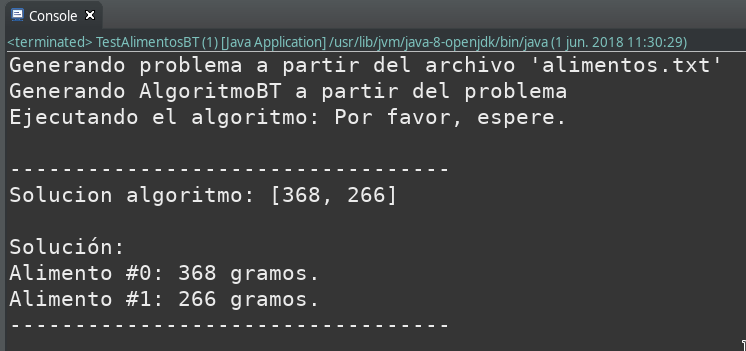
\includegraphics{btSinfiltro.png}
  \caption{Volcado de pantalla de la terminal al ejecutar la clase TestAlimentosBT}
  \label{fig:pli}
\end{figure}

\subsection{Código fuente y licencia}
Todo el código fuente del trabajo se podrá encontrar en \url{www.github.com/Andalu30/US-ADDA-PracticaIndividual2/}
a partir del lunes 4 de junio de 2018, fecha limite de entrega de este trabajo.
No se recomienda el uso de la totalidad o de parte de este trabajo en caso de que no se cambie la actividad en años posteriores debido a que la universidad usa software de detección de copias.
El contenido de este trabajo es libre y se encuentra licenciado bajo una licencia GPL v3.\\

\begin{minted}{text}
This program is free software: you can redistribute it and/or modify
it under the terms of the GNU General Public License as published by
the Free Software Foundation, either version 3 of the License, or
(at your option) any later version.

This program is distributed in the hope that it will be useful,
but WITHOUT ANY WARRANTY; without even the implied warranty of
MERCHANTABILITY or FITNESS FOR A PARTICULAR PURPOSE.  See the
GNU General Public License for more details.

You should have received a copy of the GNU General Public License
along with this program.  If not, see <http://www.gnu.org/licenses/>.

\end{minted}

\end{document}
